\indent 本研究では, シミュレーション環境を実世界により近づけるために, 
Simulation of Urban Mobility (SUMO)\cite{sumo}とOpenStreetMap\cite{openstreetmap}を利用して
岐阜駅近辺の交通データを取得し, 実際の車両の動きを再現するノードのモビリティモデルを
作成した. SUMOは都市環境における交通流動をシミュレーションするためのオープンソースソフ
トウェアである. 与えられた交通ネットワークから自動車, バス, 電車などで構成されてい
る交通流をシミュレーションすることができる. \\
\indent 移動モデル作成の手順は次の3ステップである. 
\begin{enumerate}
  \item OpenStreetMap のウェブサイトから, シミュレーションに使用したい地域の地理デ
  -タを取得する. 図\ref{fig:sumo1} はOpenStreetMapで表示した岐阜駅近辺である. Select
  Area で枠を区切り, durationでシミュレーション時間を決定し, Generate Scenario
  ボタン押すと交通流データが取得できる.\\
  \begin{figure}[h]
    \centering
    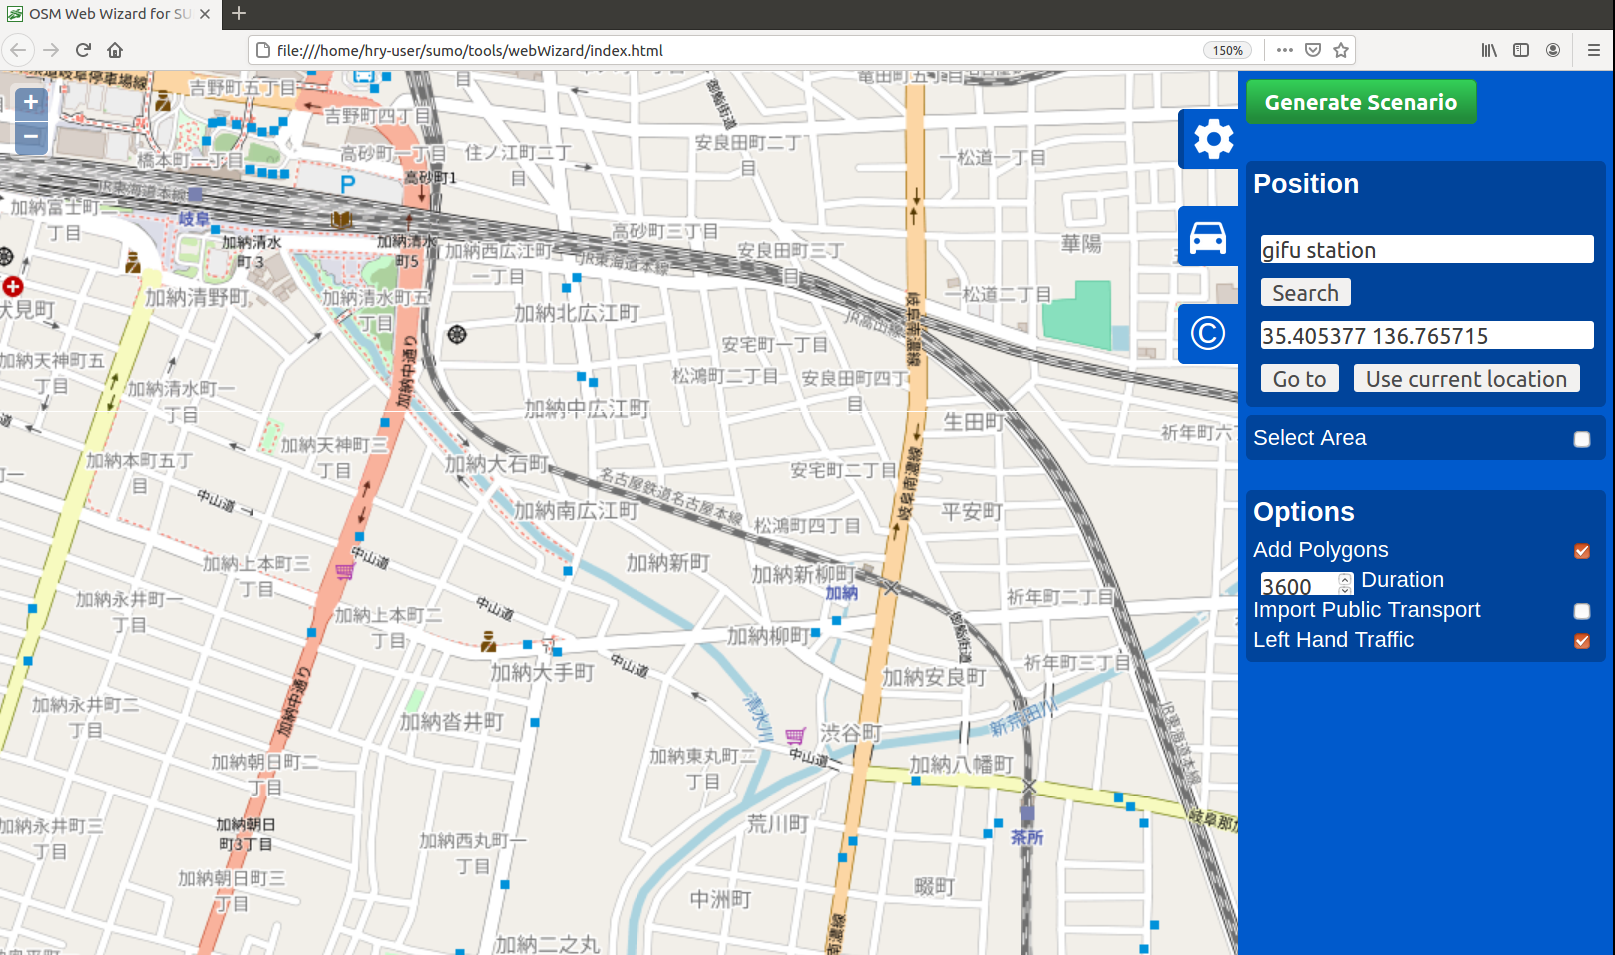
\includegraphics[scale=0.3]{figures/SUMO1.png}
    \caption{OpenStreetMapで表示した岐阜駅近辺}
    \label{fig:sumo1}
  \end{figure}
  \item OpenStreetMapで取得した地理データを, SUMO の読み取れる.xml形式に変換する. 
  このデータを用いてSUMOはシミュレーションを行う. 図\ref{fig:sumo2}は.xmlファイルに変
  換した地理データをSUMOで表示したものである. \\
  \begin{figure}[h]
    \centering
    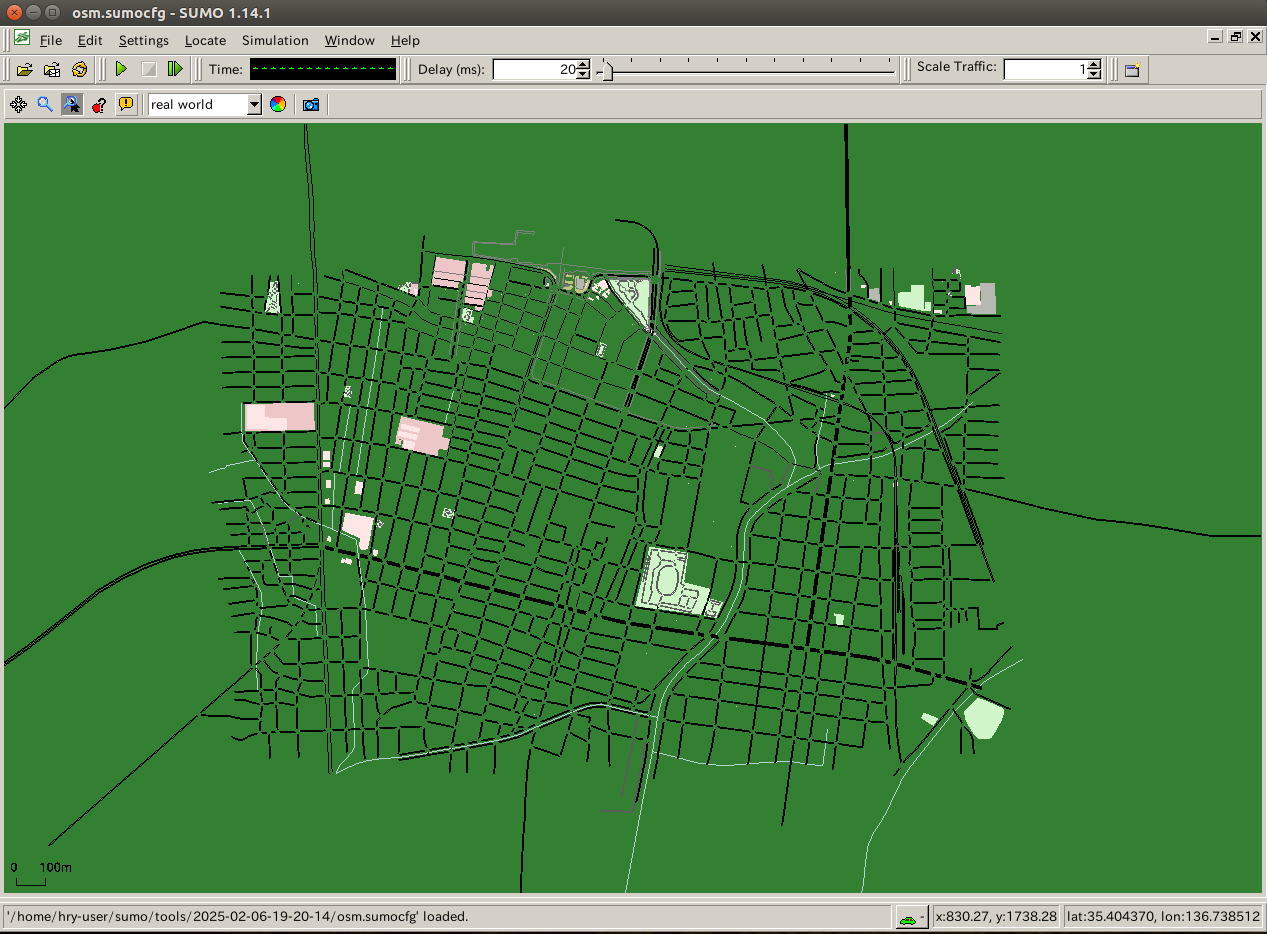
\includegraphics[scale=0.3]{figures/SUMO2.png}
    \caption{SUMOで表示した岐阜駅近辺}
    \label{fig:sumo2}
  \end{figure}
  \item SUMOで行ったシミュレーション, すなわちノードの動きのデータをns-3で読み
  取れる.tcl 形式に変換する. 図\ref{fig:sumo3}は.tcl形式に変換したノードの動きのデータを
  ns-3のビジュアライザーで表示したものである.
  \begin{figure}[h]
    \centering
    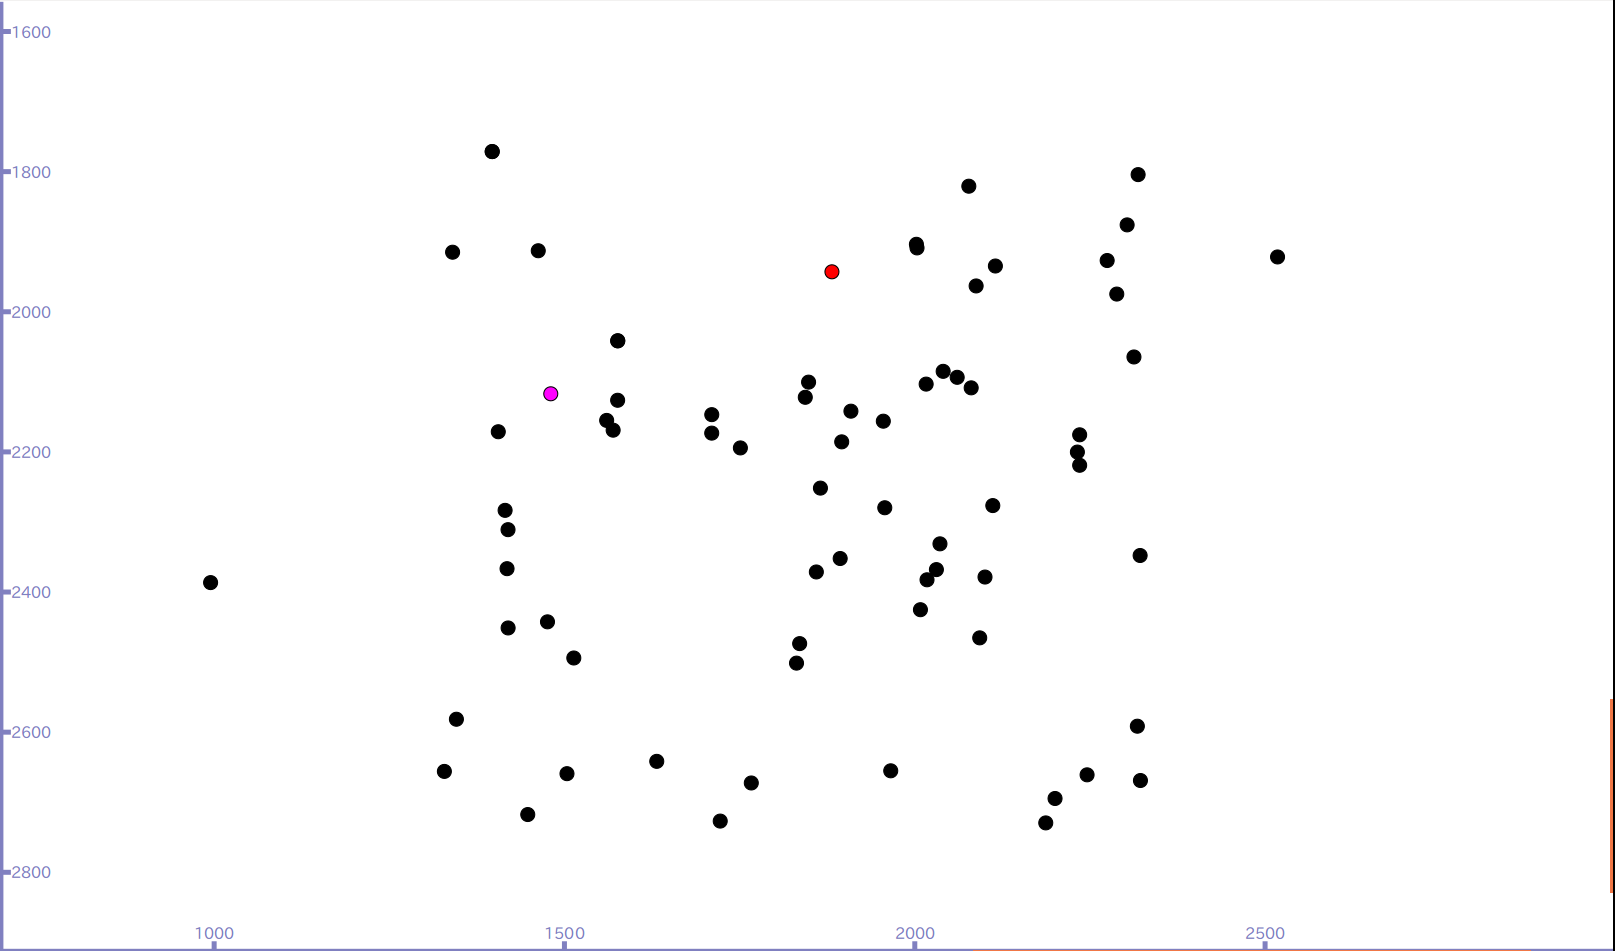
\includegraphics[scale=0.3]{figures/SUMO3.png}
    \caption{ns-3のビジュアライザーで表示した岐阜駅近辺}
    \label{fig:sumo3}
  \end{figure}

\end{enumerate}
% \indent OpenStreetMap のウェブサイトから, シミュレーションに使用したい地域の地理デ
% -タを取得する. 図\ref{fig:sumo1} はOpenStreetMapで表示した岐阜駅近辺である. Select
% Area で枠を区切り, durationでシミュレーション時間を決定し, Generate Scenario
% ボタン押すと交通流データが取得できる.\\
% \begin{figure}[t]
%   \centering
%   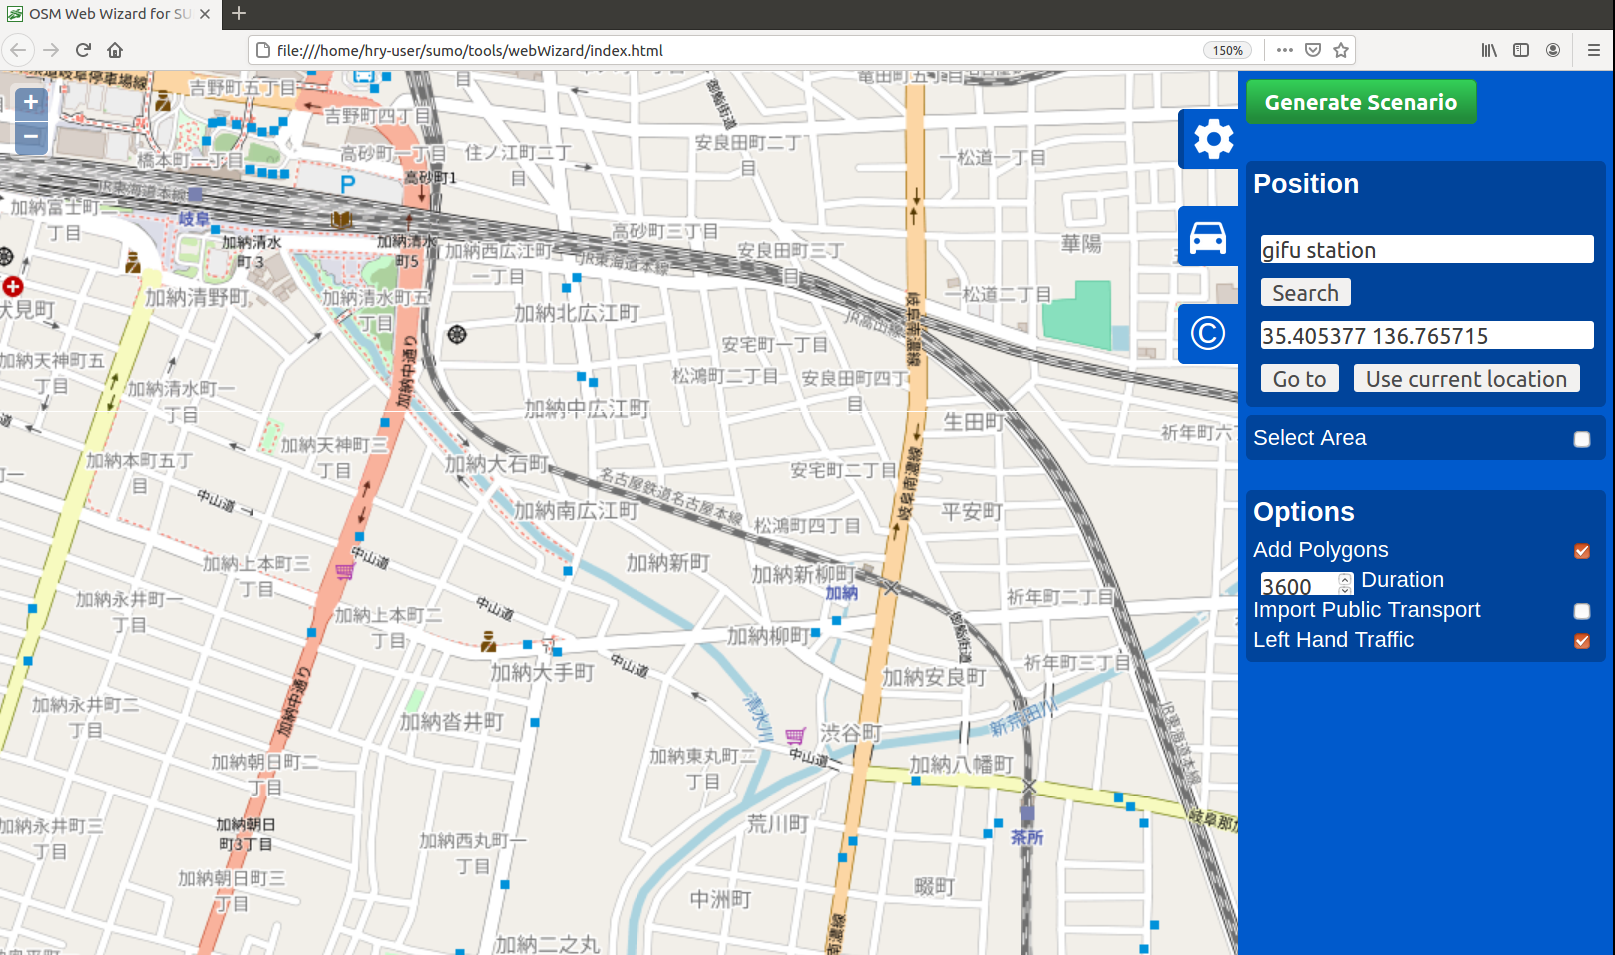
\includegraphics[scale=0.3]{figures/SUMO1.png}
%   \caption{OpenStreetMapで表示した岐阜駅近辺}
%   \label{fig:sumo1}
% \end{figure}
% \FloatBarrier
% \indent OpenStreetMapで取得した地理データを, SUMO の読み取れる.xml形式に変換する. 
% このデータを用いてSUMOはシミュレーションを行う. 図\ref{fig:sumo2}は.xmlファイルに変
% 換した地理データをSUMOで表示したものである. \\
% \begin{figure}[h]
%   \centering
%   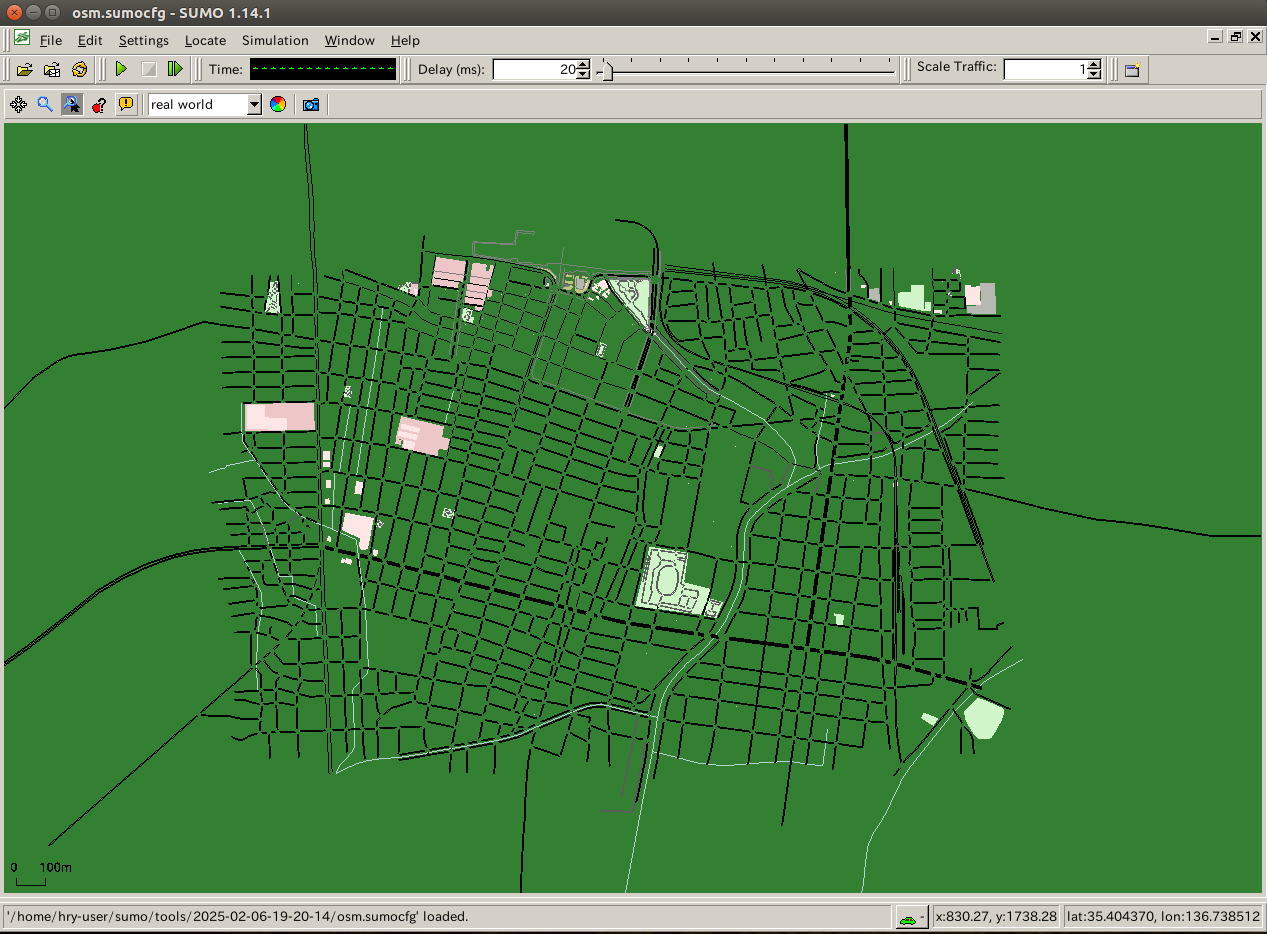
\includegraphics[scale=0.3]{figures/SUMO2.png}
%   \caption{SUMOで表示した岐阜駅近辺}
%   \label{fig:sumo2}
% \end{figure}
% \FloatBarrier
% \indent SUMOで行ったシミュレーション, すなわちノードの動きのデータをns-3で読み
% 取れる.tcl 形式に変換する. 図\ref{fig:sumo3}は.tcl形式に変換したノードの動きのデータを
% ns-3のビジュアライザーで表示したものである.
% \begin{figure}[h]
%   \centering
%   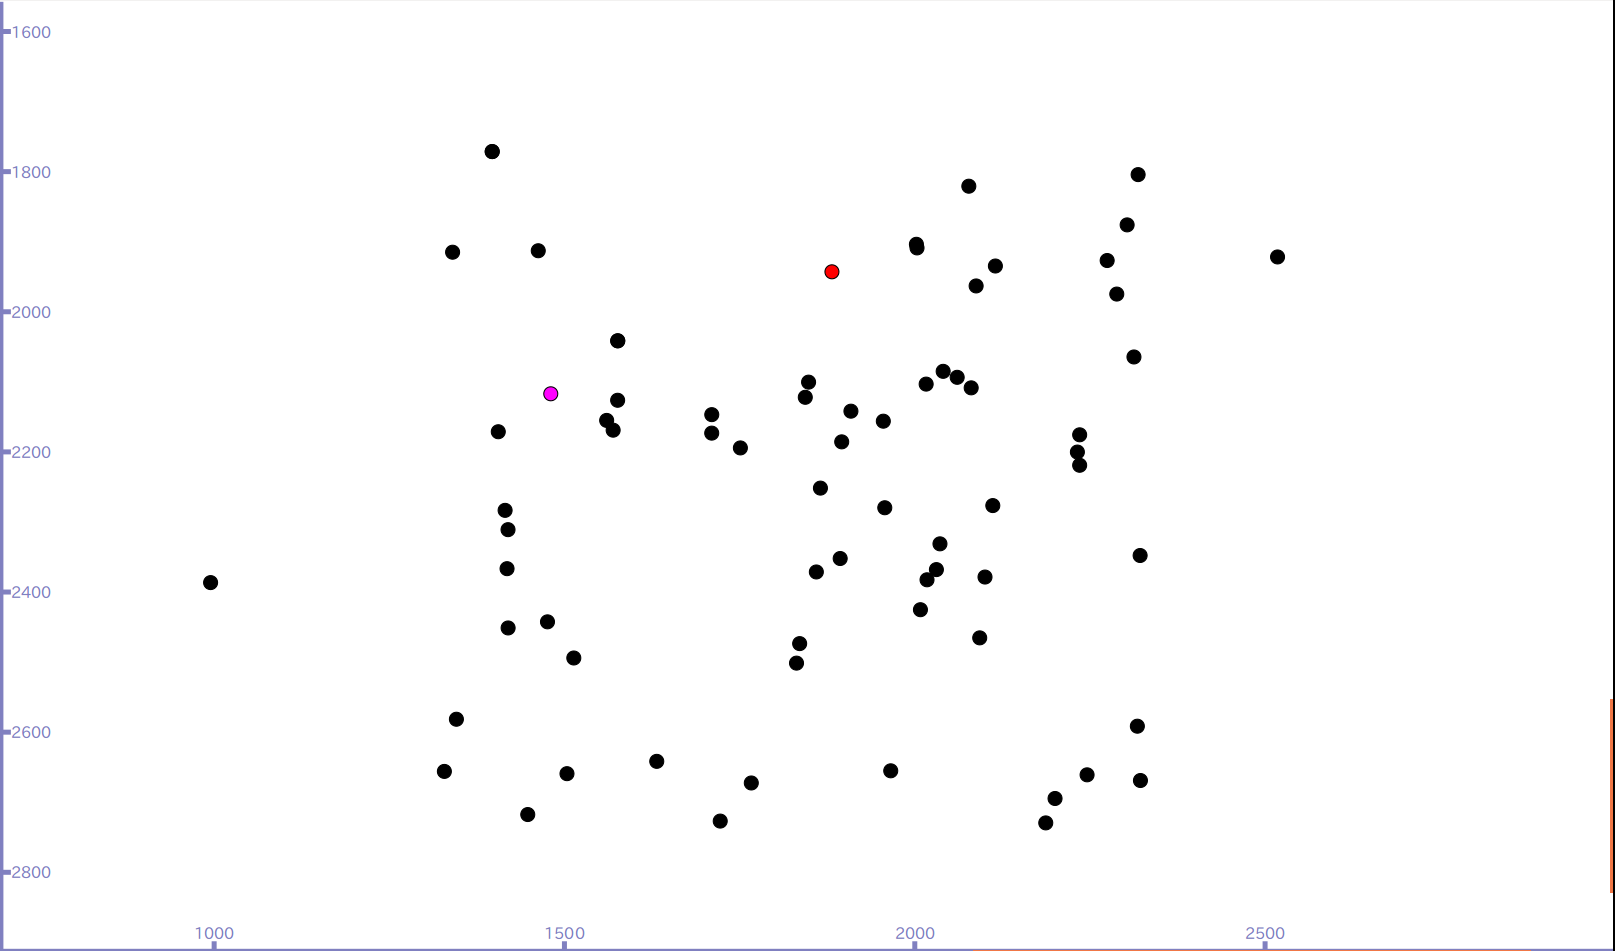
\includegraphics[scale=0.3]{figures/SUMO3.png}
%   \caption{ns-3のビジュアライザーで表示した岐阜駅近辺}
%   \label{fig:sumo3}
% \end{figure}
% \FloatBarrier
